% Main Tài liệu dùng gói ex_test, phải đi kèm file ex_test.sty 
\documentclass[12pt,a4paper,twoside]{book}
\usepackage{fouriernc}
\usepackage{amsmath,amssymb,arcs,currfile}
\usepackage{tikz,tkz-tab,tkz-linknodes,tkz-euclide,tikz-3dplot,pgfplots}
\usepackage[top=1.5cm, bottom=1.5cm, left=1.5cm, right=1.5cm] {geometry}
\usepackage[dethi]{ex_test}
% \usepackage[loigiai]{ex_test}
% \usepackage[book]{ex_test}
% \usepackage[color]{ex_test}
% \usepackage[solcolor]{ex_test}
%\input{C:/texlive/Khai-bao-cho-file-main}
% \renewcommand{\baselinestretch}{1.2}
%%%%%%%%%%%%%%%%%\
\begin{document}
	\Opensolutionfile{ans}
	%-------------------------
	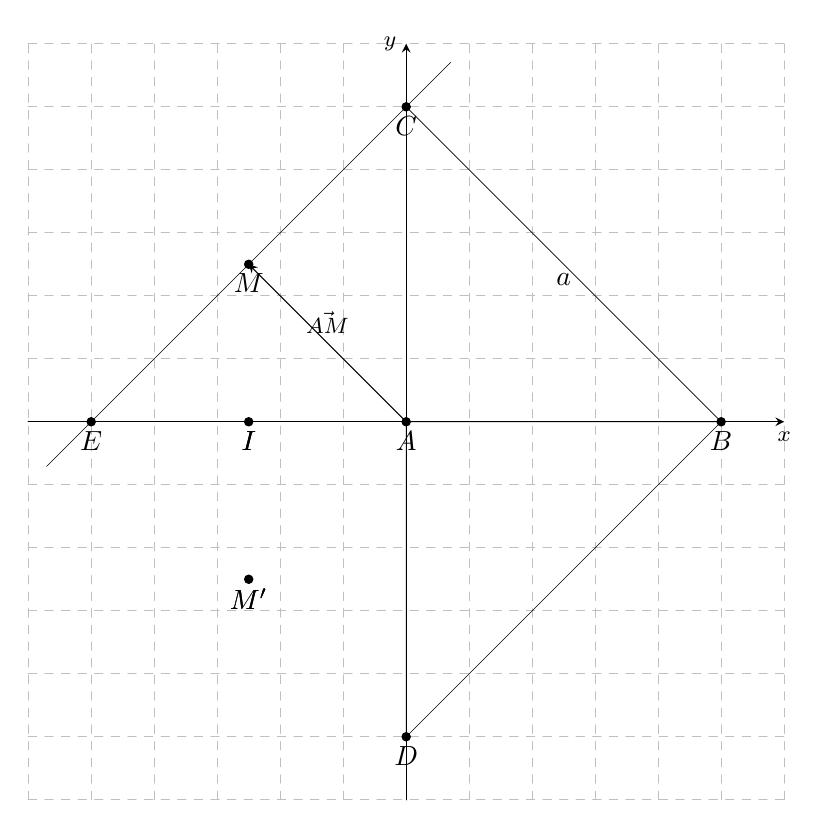
\begin{tikzpicture}[scale=0.8,>=stealth, font=\footnotesize, line join=round, line cap=round]
		\draw[color=gray!50,dashed] (-6,-6) grid (6,6);
		\draw[->] (-6,0)--(6,0) node [below]{$x$};
		\draw[->] (0,-6)--(0,6) node [left]{$y$};
		\clip (-6,-6) rectangle (6,6);
		%%%%%%%%%%%%%%%
		\tkzDefPoints{0/0/A,5/0/B,0/5/C,0/-5/D,-5/0/E}
		\tkzLabelPoints[below](A)
		\tkzLabelPoints[below](B)
		\tkzLabelPoints[below](C)
		\tkzLabelPoints[below](D)
		\tkzLabelPoints[below](E)
		\tkzLabelSegment(C,B){$a$}

		
		
		\tkzDrawPoints[fill=black,size=3](A,B,C,D,E)
		\tkzDrawSegments(B,C)
		\tkzDrawLines[add=1cm and 1cm](C,E)
		\tkzDrawPolygon(A,B,D)
		\coordinate (I) at ($(A)!0.5!(E)$);
		
		\tkzLabelPoints[below](I)
		\coordinate (M) at ($(E)!0.5!(C)$);
		\coordinate (M) at ($(E)!0.5!(C)$);
		
		
		\coordinate (M') at ($(I)!-1!(M)$);
		\tkzLabelPoints[below](M')
		
		\tkzDrawPoints[fill=black,size=3](M,I,M')
		\tkzLabelPoints[below](M,I,M')
	
		\draw[->,>=stealth] (A) -- (M) node[midway, above] {$\vec{AM}$};
		
		
		\end{tikzpicture}
		\vspace{1cm}	
	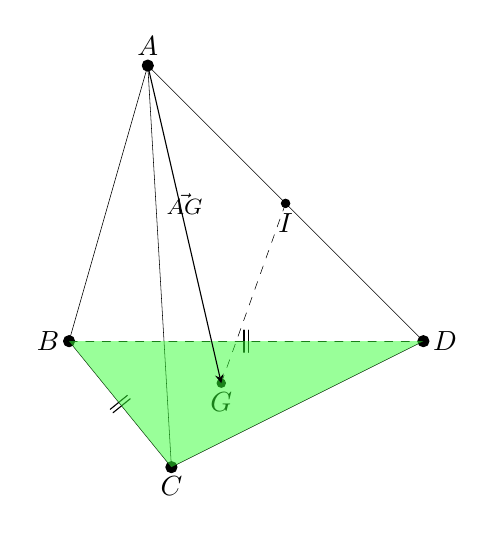
\begin{tikzpicture}[scale=1,>=stealth, font=\footnotesize, line join=round, line cap=round]
		\tkzDefPoints{0/0/B,1.3/-1.6/C,4.5/0/D,1/3.5/A}
		\tkzDrawPolygon(A,B,C,D)
		\tkzDrawSegments(A,C)
		\tkzDrawSegments[dashed](B,D)
		\tkzDrawPoints[fill=black,size=4](A,B,C,D)
		\tkzLabelPoints[above](A)
		\tkzLabelPoints[below](C)
		\tkzLabelPoints[left](B)
		\tkzLabelPoints[right](D)
		\tkzCentroid(D,B,C)\tkzGetPoint{G}
		\tkzDrawPoints[fill=black,size=3](G)
		\tkzLabelPoints[below](G)
		\coordinate (I) at ($(A)!0.5!(D)$);
		\tkzDrawPoints[fill=black,size=3](I)
		\tkzLabelPoints[below](I)
		\tkzDrawSegments[dashed](G,I)
		\tkzMarkSegments[mark=||](B,C B,D)
		\tkzFillPolygon[color=green!80, fill opacity=0.5](B,C,D)
		\draw[->,>=stealth] (A) -- (G) node[midway, above] {$\vec{AG}$};

		
	\end{tikzpicture}
	

	
	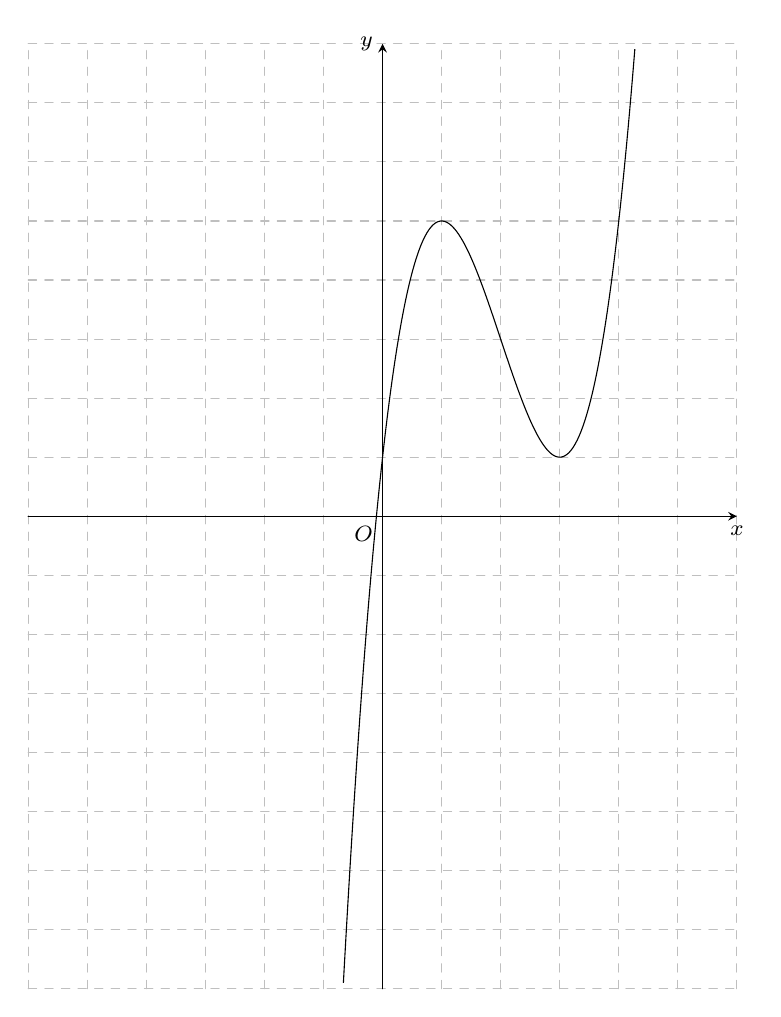
\begin{tikzpicture}[scale=0.75,>=stealth, font=\footnotesize, line join=round, line cap=round]
		\def\a{1} \def\b{-6} \def\c{9} \def\d{1} % Hệ số
		\def\xmin{-6} \def\xmax{6}
		\def\ymin{-8} \def\ymax{8} 
		\draw[color=gray!50,dashed] (\xmin,\ymin) grid (\xmax,\ymax); 
		\draw[->] (\xmin,0)--(\xmax,0) node [below]{$x$};
		\draw[->] (0,\ymin)--(0,\ymax) node [left]{$y$};
		\node at (0,0) [below left]{$O$};
		\clip (\xmin+0.1,\ymin+0.1) rectangle (\xmax-0.5,\ymax-0.1);
		\draw[smooth,samples=300] plot(\x,{\a*(\x)^3+\b*(\x)^2+\c*(\x)+\d});
	\end{tikzpicture}
	%-------------------------
	\Closesolutionfile{ans}
	
\end{document}